\documentclass[../main.tex]{subfiles}
\graphicspath{{\subfix{../figures/}}}
\begin{document}

\section{$\nu_{\mu}$ CC $\pi^{0}$ Selection}
\label{sec:selection}


\subsection{Signal Definition}
The $\nu_{\mu}$ CC $\pi^{0}$ signal definition encompasses charged-current neutrino interactions occuring within the fiducial volume of the detector and containing
\begin{itemize}
    \item exactly one primary muon ($p_{\mu} \ge 226$ MeV/c)
    \item exactly zero primary charged pions ($E_{\pi^{\pm}} \ge 25$ MeV)
    \item exactly one primary neutral pion
    \item any number of particles that are not muons or pions.
\end{itemize}
The momentum/energy requirements for muons and charged pions are phase space constraints to ensure tracking thresholds are met and purity is optimized.  This signal definition applies to final state particles, or particles exiting the target nucleus post-final state interactions (FSI).  The fiducial volume requirement applies to the neutrino interaction vertex, which must be 25 cm from detector boundaries in the drift and vertical directions, 30 cm from the upstream detector face, and 50 cm from the downstream face.

\subsection{Selection Cuts}
When selecting $\nu_{\mu}$ CC $\pi^{0}$ interactions, cuts are made on various reconstructed outputs to narrow the list of candidate interactions.  Included are cuts on:
\begin{itemize}
    \item \underline{Fiducial volume}: Reconstructed vertex is required to be inside fiducial volume (defined in signal definition).
    \item \underline{Flash time}: Interaction is associated with an optical flash that is in-time with BNB beam gate, as determined by the OpT0Finder algorithm.
    \item \underline{Base Topology}: Interaction contains
        \begin{itemize}
            \item Exactly one primary muon ($p_{\mu} \ge 226$ MeV/c)
            \item Exactly zero primary charged pions ($E_{\pi^{\pm}} \ge 25$ MeV)
            \item Two or three primary photons ($E_{\gamma} \ge 20$ MeV)
        \end{itemize}
    \item \underline{Leading Photon}: Highest energy photon has $E_{\gamma} \ge 40$ MeV
    \item \underline{Neutral pion mass}: Invariant diphoton mass $<$ 400 MeV in order to reject $\eta$ mesons.
\end{itemize}
Note that in the case of three primary photons meeting the above selection criteria, the photon pair with diphoton invariant mass closest to that of the true $\pi^{0}$ mass is chosen to belong to the candidate $\pi^{0}$.

\subsection{Selection Performance}
Selection performance is assessed using the BNB $\nu$ + Cosmic MC sample and off-beam BNB Run 2 data.  The metrics that have been evaulated are efficiency - the fraction of true signal interactions that are matched to selected interactions, and purity - the fraction of selected interactions that are matched to true signal interactions.  Efficiency and purity for each selection cut are shown in Table \ref{Tab:pureff}.

\begin{table}[H]
    \caption{Purity and efficiency for $\nu_{\mu}$ CC $\pi^{0}$ Selection Cuts}
    \vspace{0.1cm}
    \centering
    \begin{tabular}{ c c c } 
    \hline
    Selection Cut & Efficiency [\%] & Purity [\%]  \\
    \hline
    No Cut & 100.0 & 0.0 \\ 
    In-Time Flash & 97.1 & 0.5 \\
    Fiducial Volume & 96.6 & 2.6 \\
    Base Topology & 71.6 & 80.7 \\
    Leading Shower & 71.6 & 81.1 \\
    $m_{\gamma \gamma} < 400$ MeV/c$^{2}$ & \textbf{71.5} & \textbf{82.6} \\
    \hline
    \end{tabular}
    \label{Tab:pureff}
\end{table}

Selection efficiency as a function of the cross section variables introduced in Section 1 are shown in Figure \ref{fig:sel_efficiency_plots}, showing that efficiency is largely flat across the signal phase space.  Both inefficiencies and impurities in the selection are driven by particle identification (PID) failures, as shown in confusion matrices for true signal particles (Figure \ref{fig:sel_pid_confusion}a) and reconstructed selected particles (Figure \ref{fig:sel_pid_confusion}b).  Background topologies are further discussed in Section 2.4.

\begin{figure}[H]
    \center
    \subfloat[True muon momentum.]{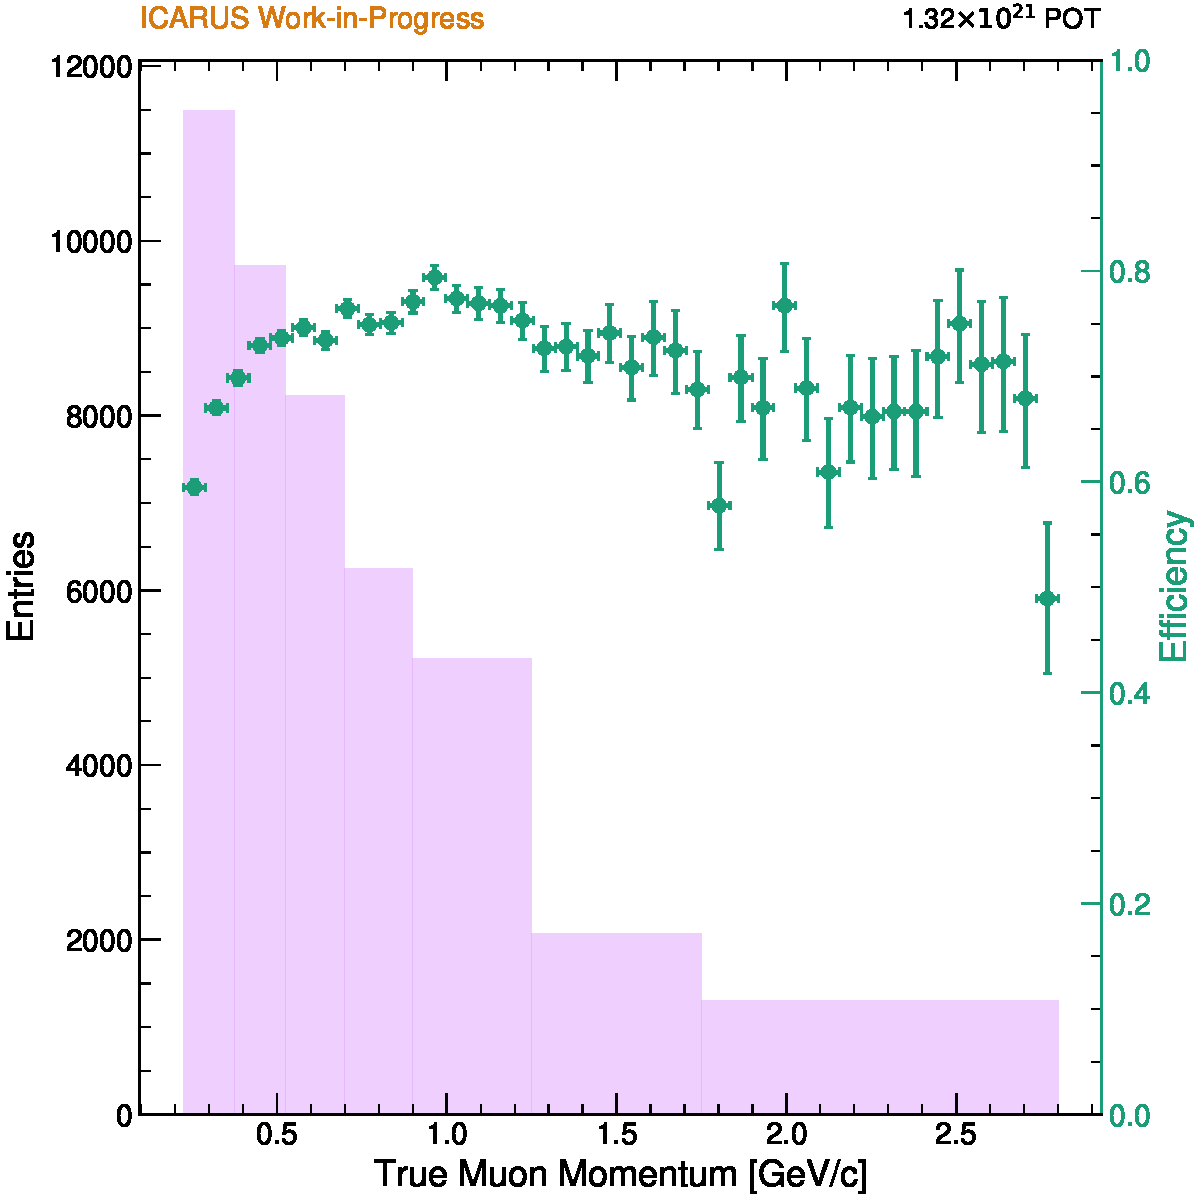
\includegraphics[width=0.50\textwidth]{eff_vs_true_muon_momentum_mag.pdf}}
    \subfloat[True $\cos{\theta_{\mu}}$.]{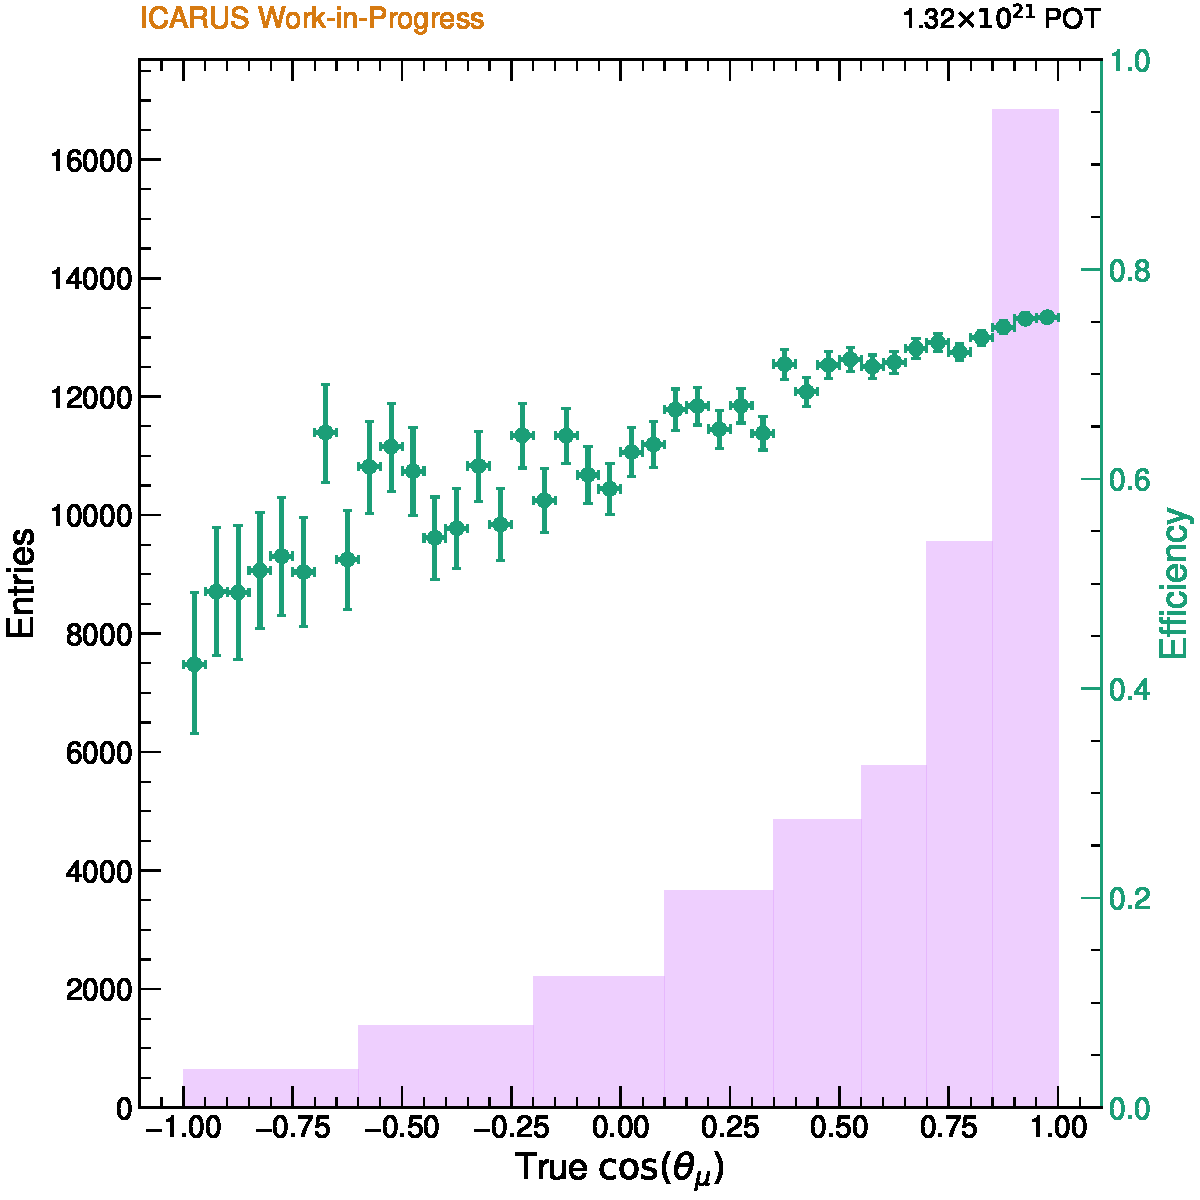
\includegraphics[width=0.50\textwidth]{eff_vs_true_muon_beam_costheta.pdf}} \\
    \subfloat[True neutral pion momentum.]{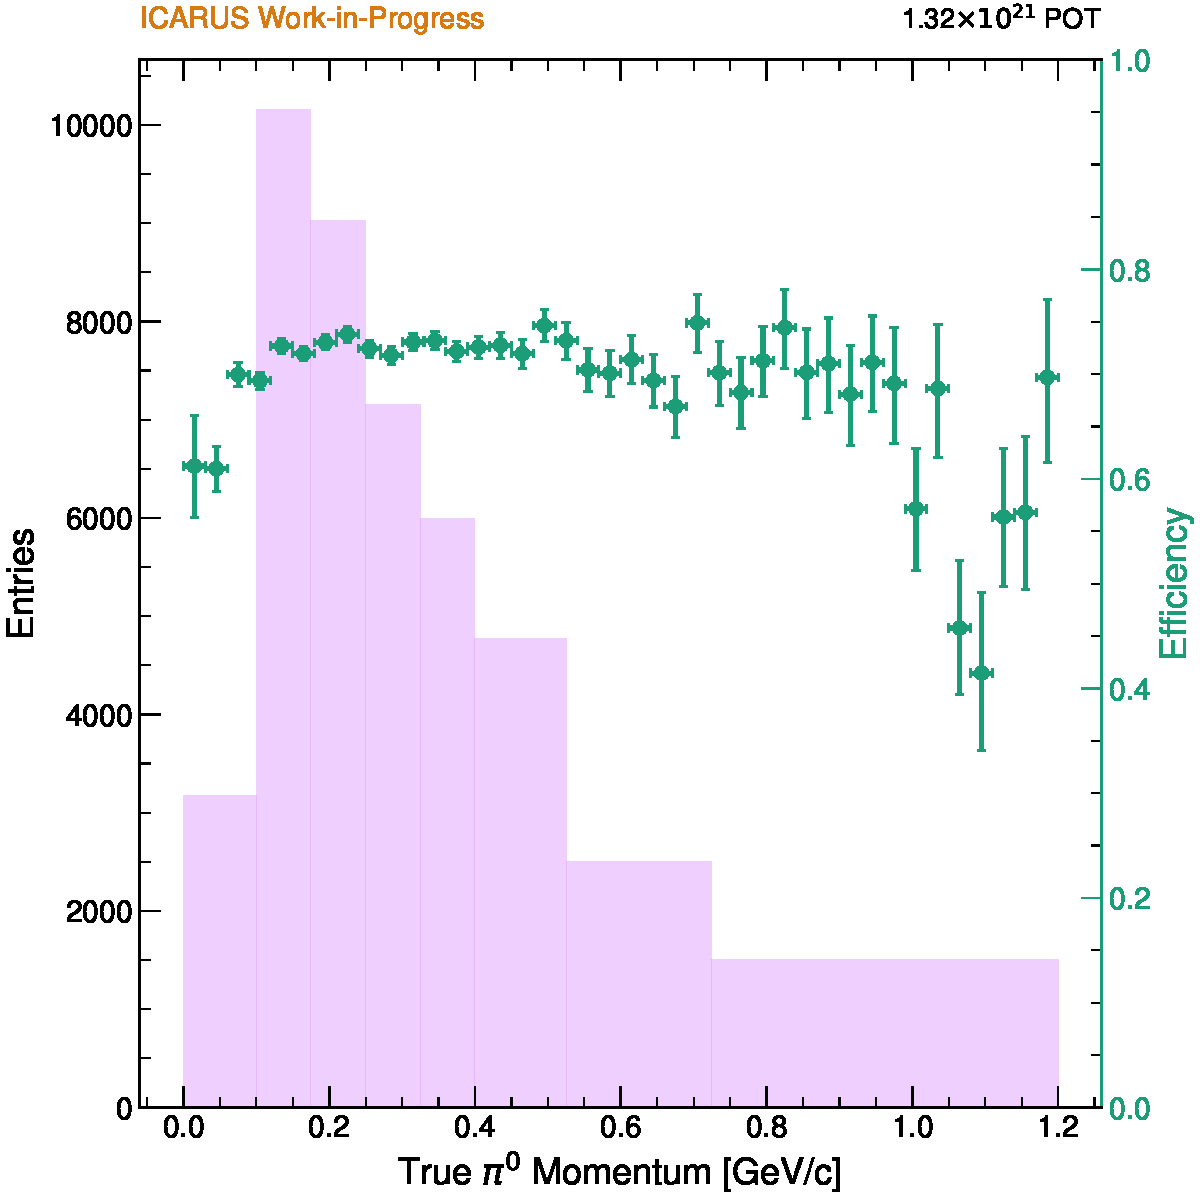
\includegraphics[width=0.50\textwidth]{eff_vs_true_pi0_momentum_mag.pdf}}
    \subfloat[True $\cos{\theta_{\pi^{0}}}$.]{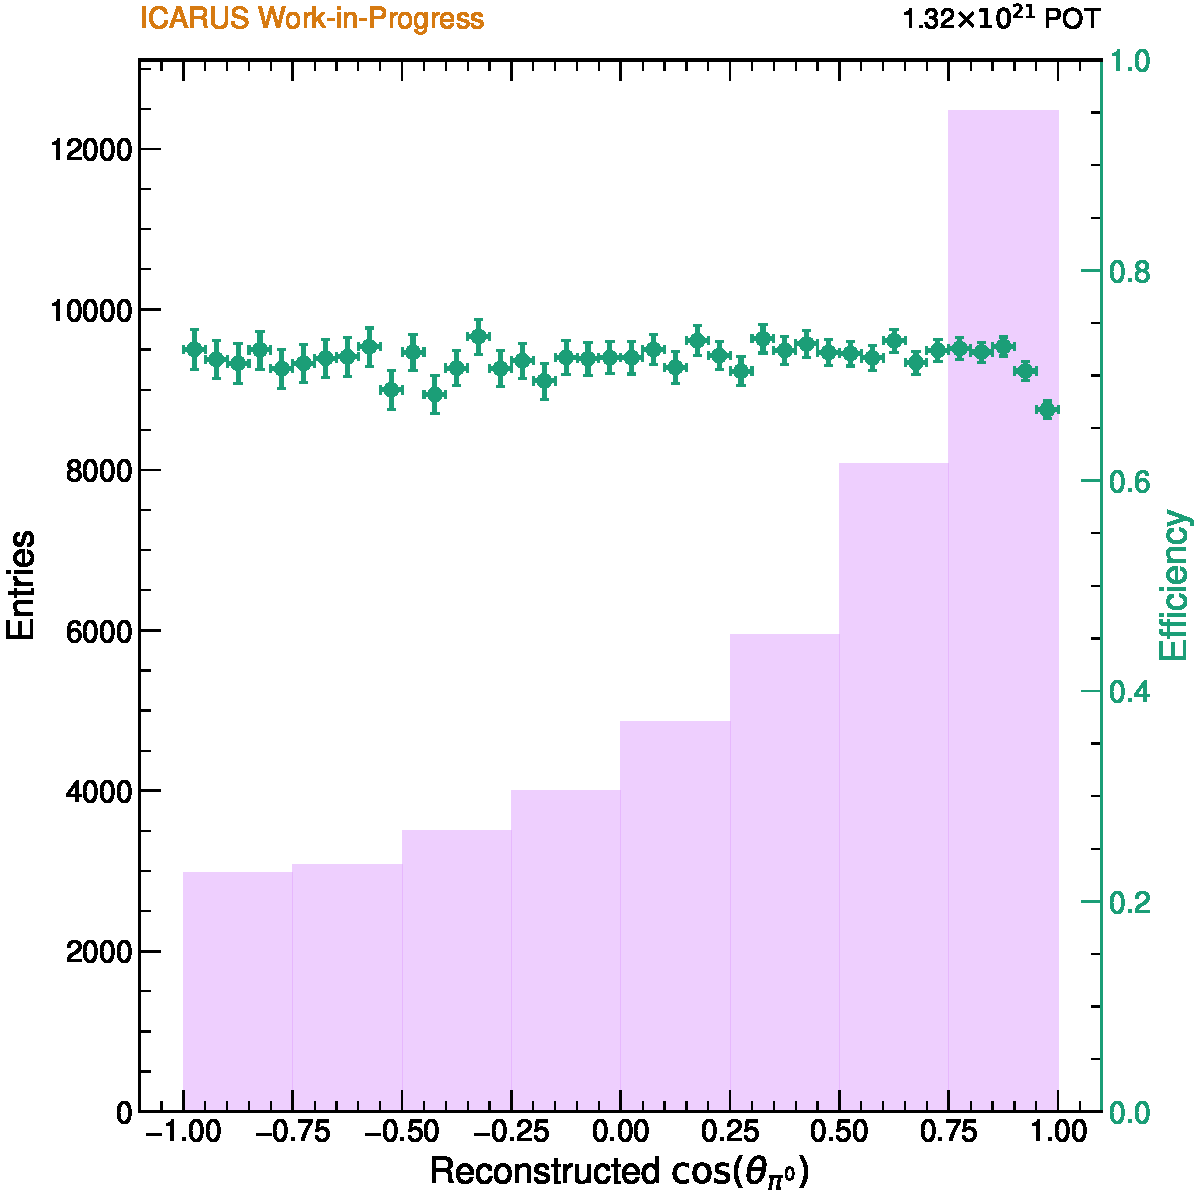
\includegraphics[width=0.50\textwidth]{eff_vs_true_pi0_beam_costheta.pdf}}
    \caption{Confusion matrices for particle identification, as determined by the SPINE machine-learning chain.}
    \label{fig:sel_efficiency_plots}
\end{figure}

\begin{figure}[H]
    \center
    \subfloat[True-to-reco matching.]{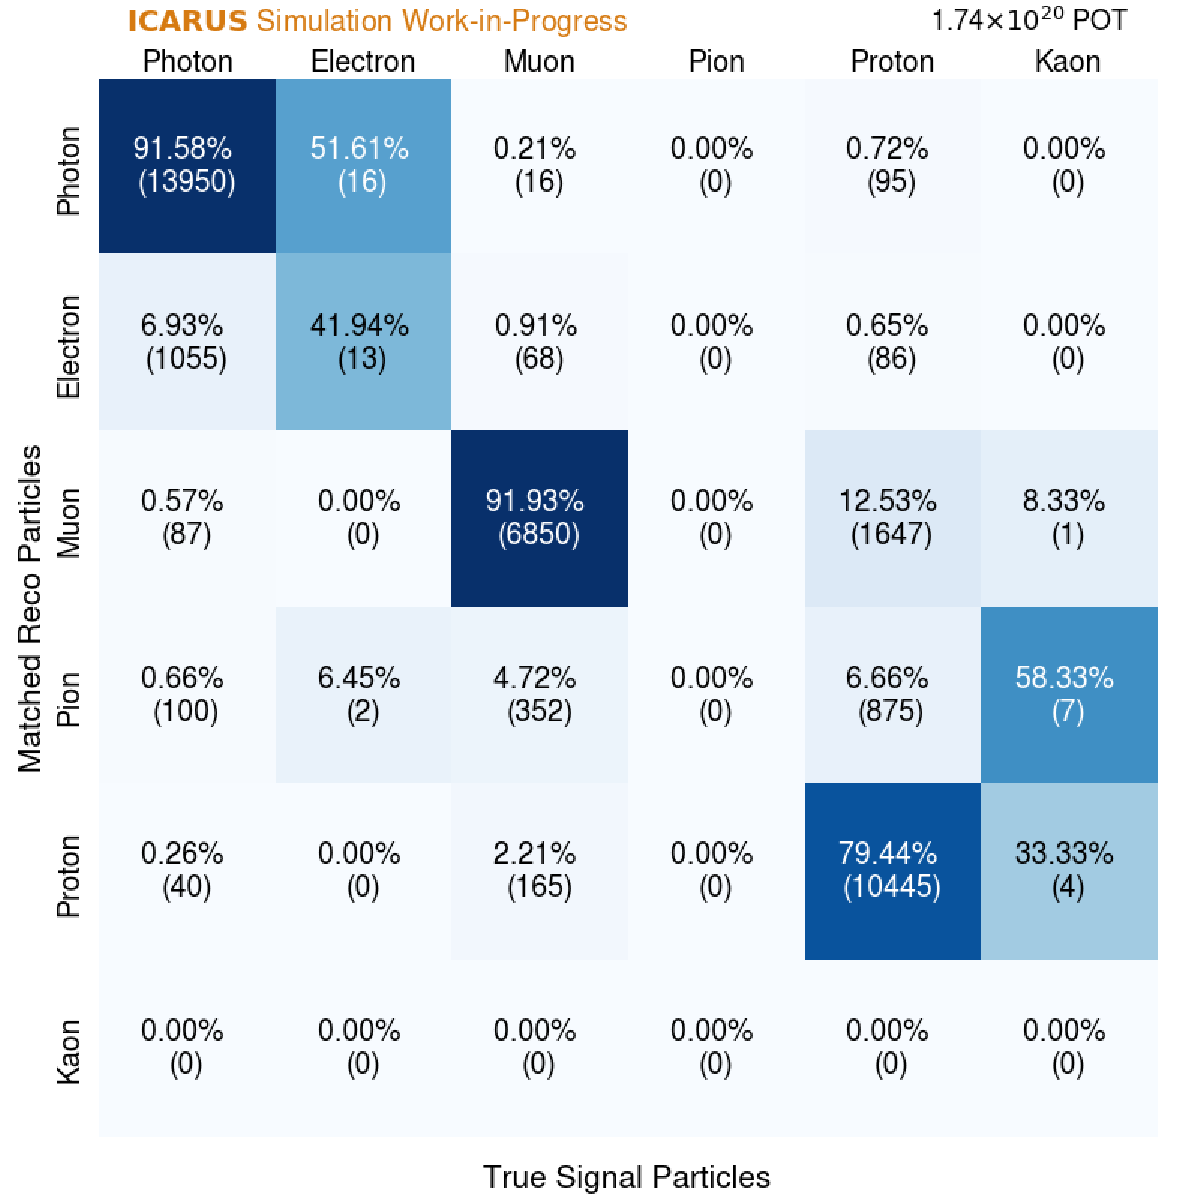
\includegraphics[width=0.50\textwidth]{eff_pid_confusion.pdf}}
    \subfloat[Reco-to-true matching.]{
\includegraphics[width=0.50\textwidth]{missing.pdf}} 
    \caption{Confusion matrices for particle identification, as determined by the SPINE machine-learning chain.}
    \label{fig:sel_pid_confusion}
\end{figure}

\subsection{Reconstructed Observables}
\label{subsec:vars}
In this section, the kinematic observables used in the single differential cross section measurement are highlighted.  Included are the momenta of the final state muon and neutral pion, as well as the angles these particles make with the BNB.  An additional variable, the invariant diphoton mass, is examined as it serves as a useful standard candle in the calibration of the electromagnetic shower energy scale.

\subsubsection{Muon Observables}
\begin{figure}[H]
    \center
    \subfloat[Muon momentum]
        {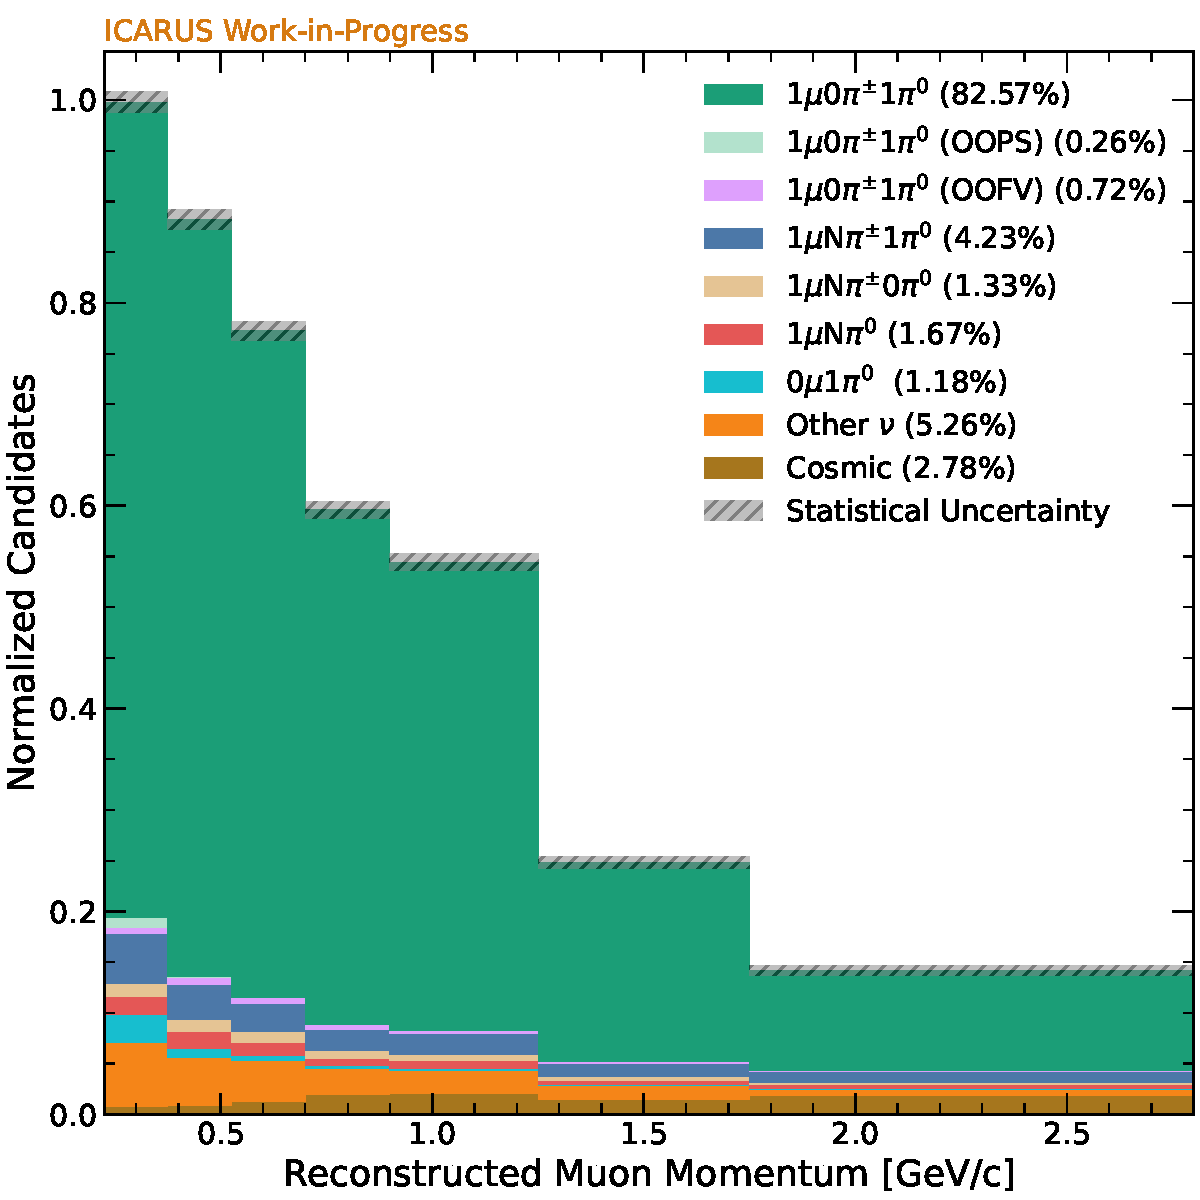
\includegraphics[width=0.50\textwidth]{reco_muon_momentum_mag.pdf} \label{subfig:reco_muon_momentum_mag}}
    \subfloat[Muon angle with respect to neutrino beam]
        {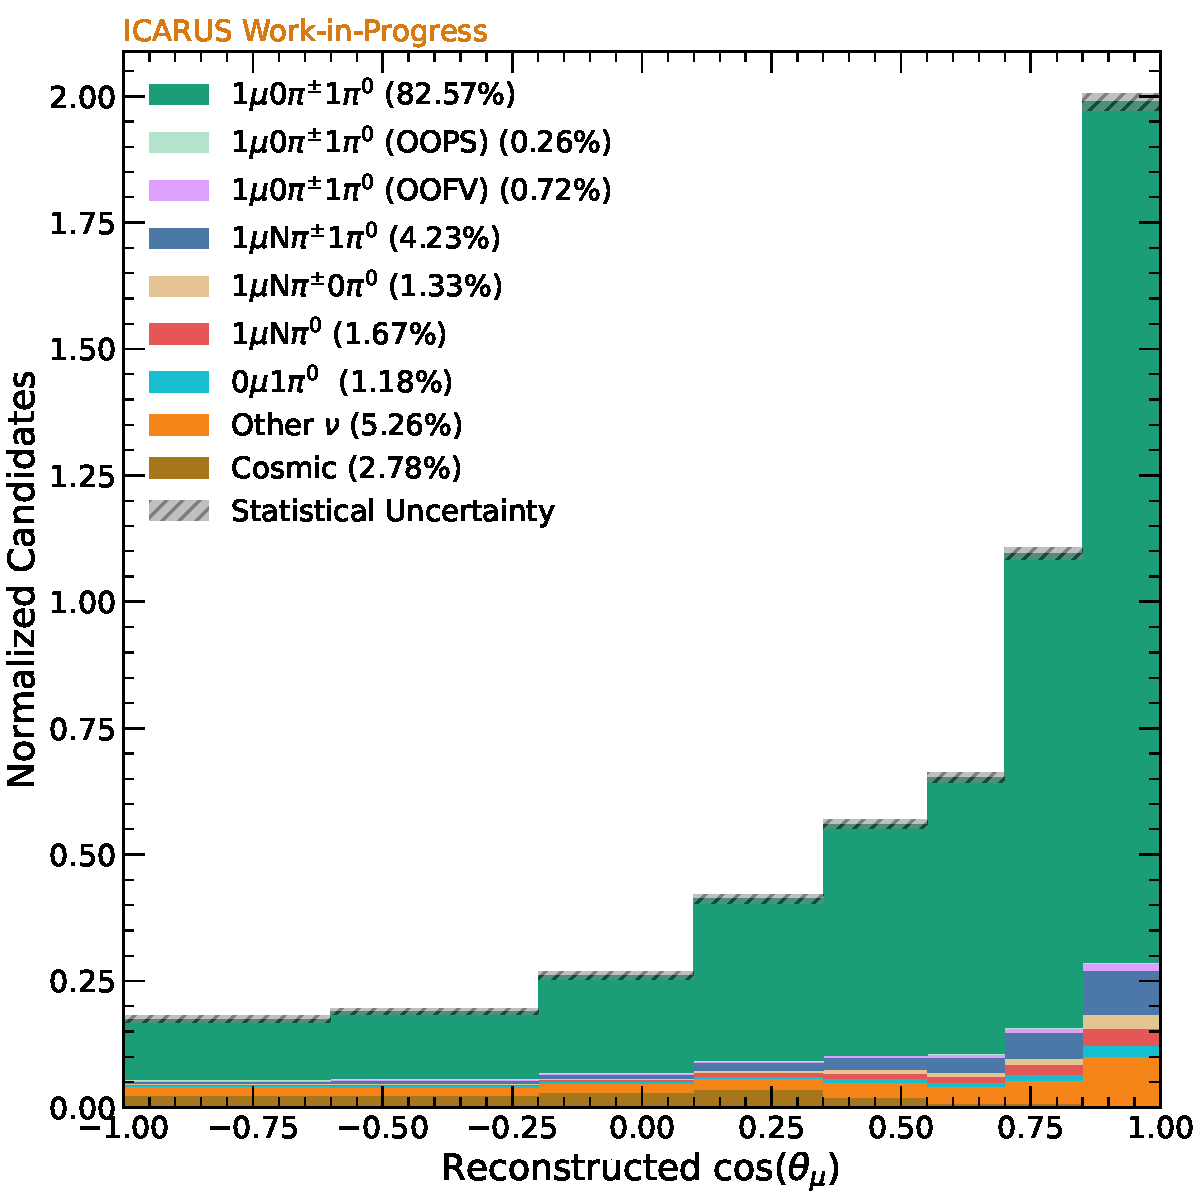
\includegraphics[width=0.50\textwidth]{reco_muon_beam_costheta.pdf} \label{subfig:reco_muon_beam_costheta}}
    \caption{Muon observables chosen for analysis}
    \label{fig:reco_muon_observables}
\end{figure}

\subsubsection{Neutral Pion Observables}
\begin{figure}[H]
    \center
    \subfloat[Neutral pion momentum]
        {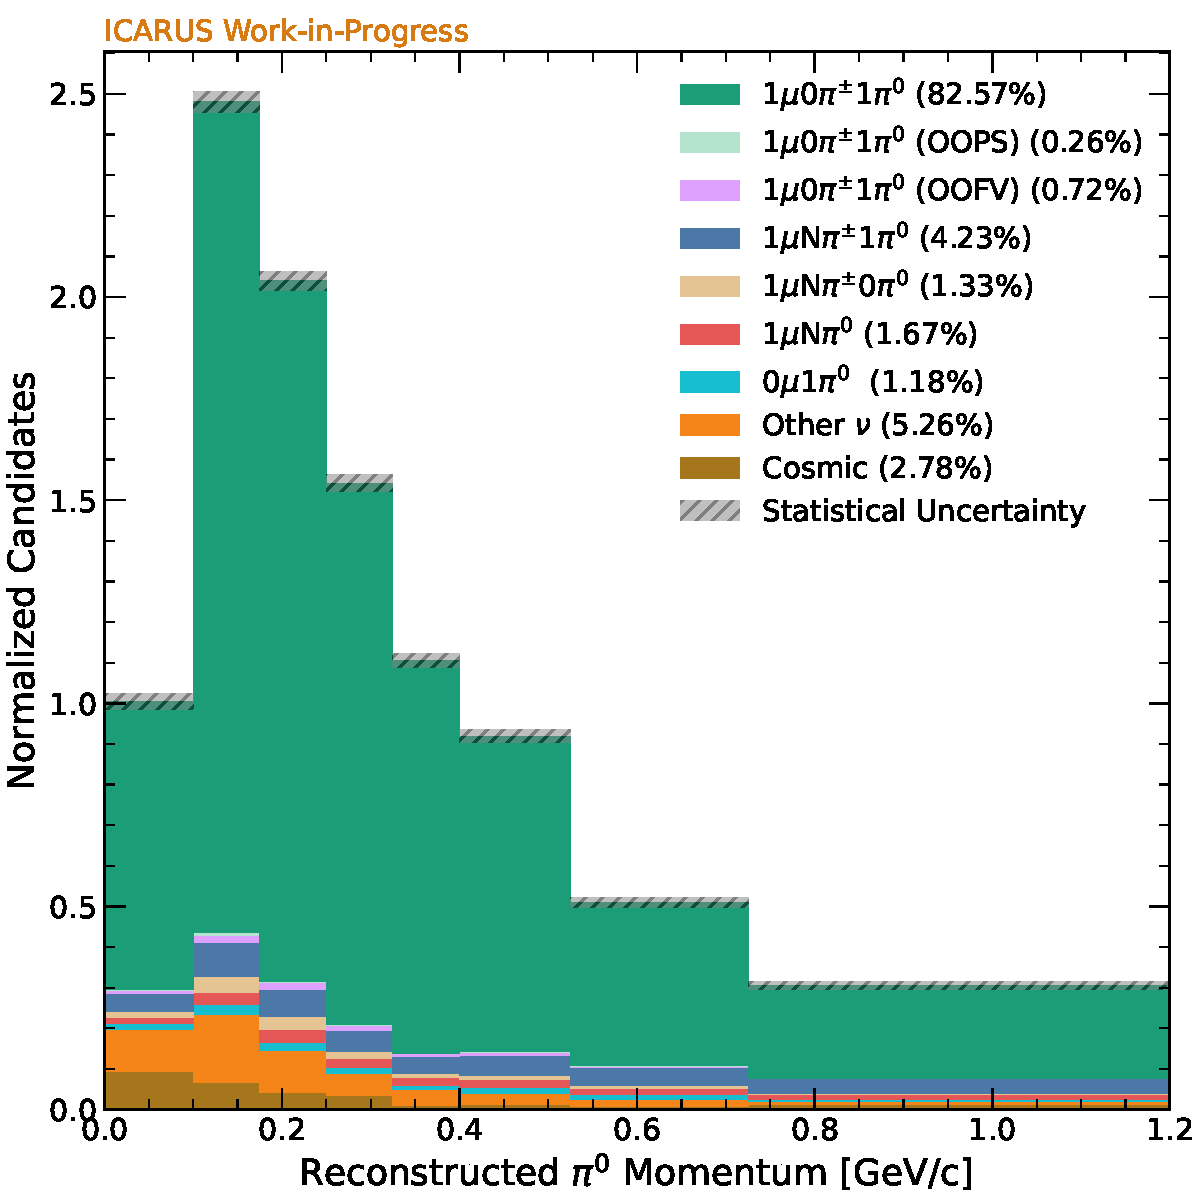
\includegraphics[width=0.50\textwidth]{reco_pi0_momentum_mag.pdf} \label{subfig:reco_pi0_momentum_mag}}
    \subfloat[Neutral pion angle with respect to neutrino beam]
        {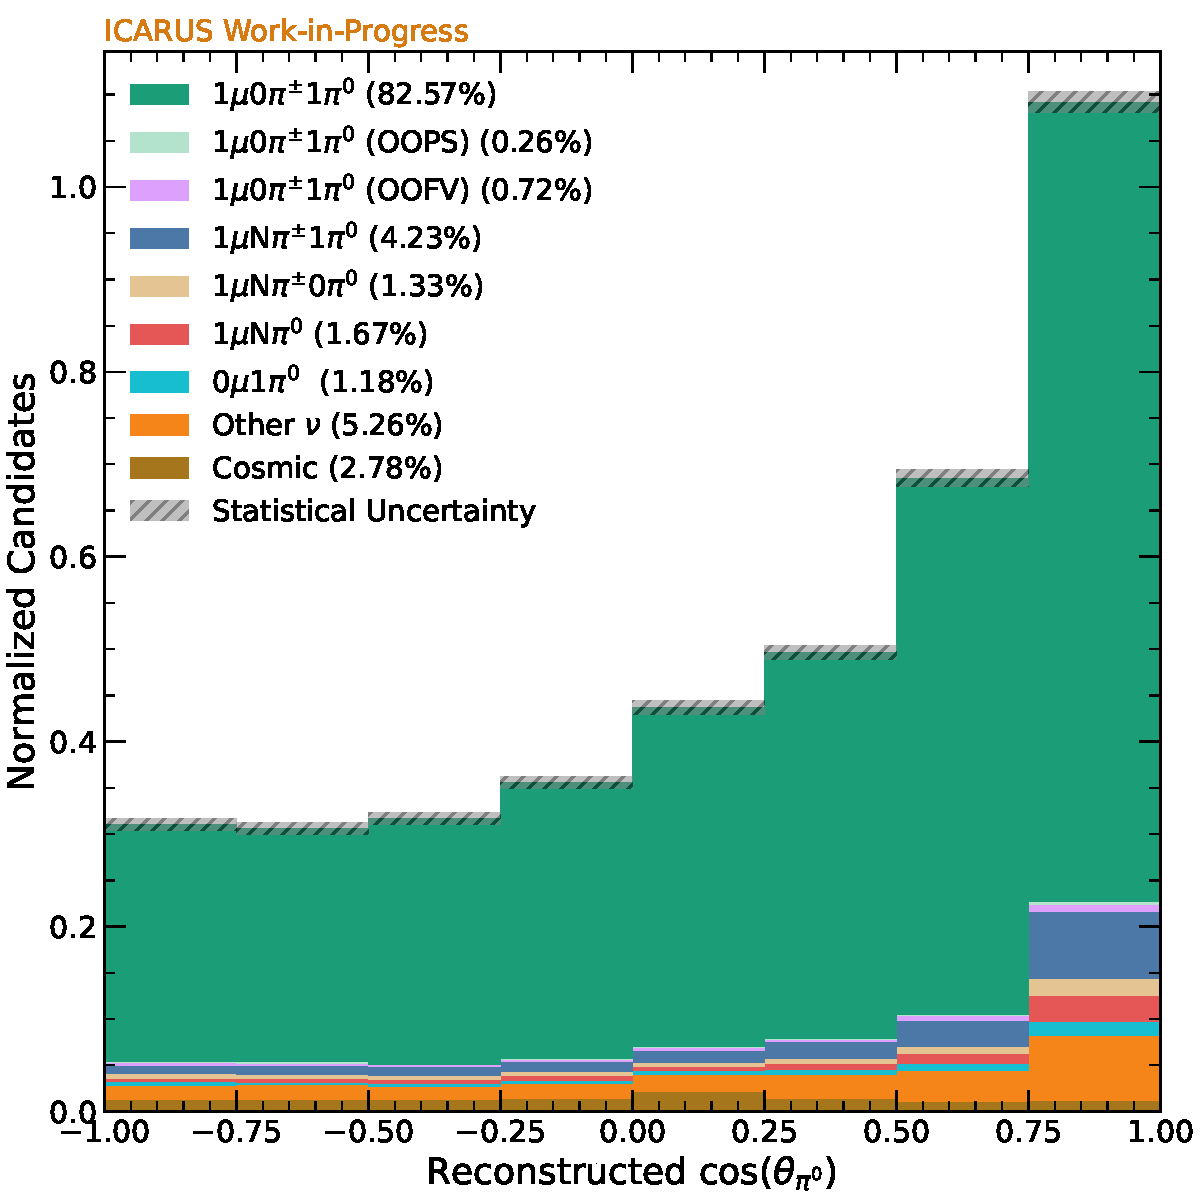
\includegraphics[width=0.50\textwidth]{reco_pi0_beam_costheta.pdf} \label{subfig:reco_pi0_beam_costheta}}
    \caption{Neutral pion observables chosen for analysis}
    \label{fig:reco_pi0_observables}
\end{figure}

\begin{figure}[H]
    \center
    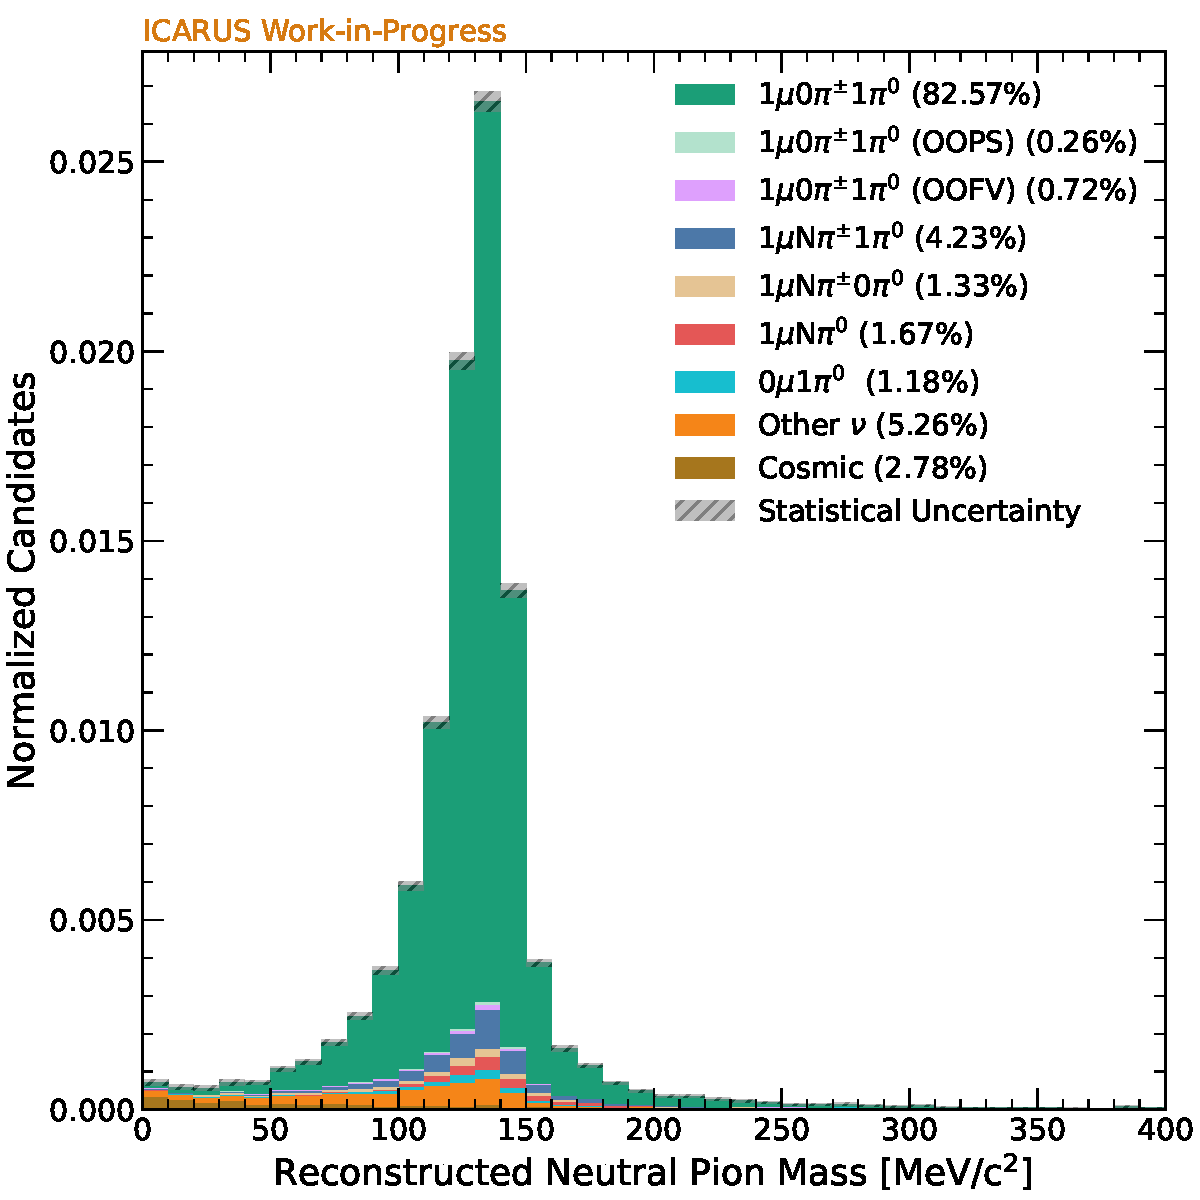
\includegraphics[width=0.90\textwidth]{reco_pi0_mass.pdf}
    \caption[text]{Neutral pion invariant mass}
    \label{fig:reco_pi0_mass}
\end{figure}


\end{document}